\chapter{Introducción}


\begin{itemize}
  \item \itembf{lista}
  \item \itembf
  \item \itembf
  \item \itembf
  \item \itembf
\end{itemize}

\textbf{``astronomía''}:


\begin{quote}``\textit{cita cita cita}''
\newline(\href{https://www.google.es}{Google})
\end{quote}




\section{Motivación y análisis del problema}
\bigskip
Como ya hemos hablado en el capítulo anterior, {\titulo} viene de una aplicación móvil híbrida en la que se detectaron carencias que probablemente provengan de la inexperiencia y el escaso tiempo de análisis del que se disponía. Vamos a exponer brevemente las características de las aplicaciones híbridas para entender los problemas que este proyecto pretende solventar.

\subsection{Aplicaciones móviles híbridas}
Con la llegada de los \textit{smartphone} se ha impulsado enormemente el consumo y producción de apps móviles. En un principio, una aplicación móvil se desarrollaba como aplicación nativa con los contras que ello supone, como una curva de aprendizaje alta de un sistema concreto, en la mayoría de los casos desarrollo monoplataforma, y también los pros como un desarrollo y control mas específico del sistema, sistemas mas robustos,etc.

\bigskip
Ni que decir tiene que una aplicación compleja necesita las ventajas de un desarrollo específico y nativo de un sistema móvil, pero ¿qué pasa con las aplicaciones simples y livianas que, cada vez más, consumimos? Es aquí donde toman importancia las aplicaciones móviles híbridas.

\begin{figure}[!ht]
  \begin{center}
  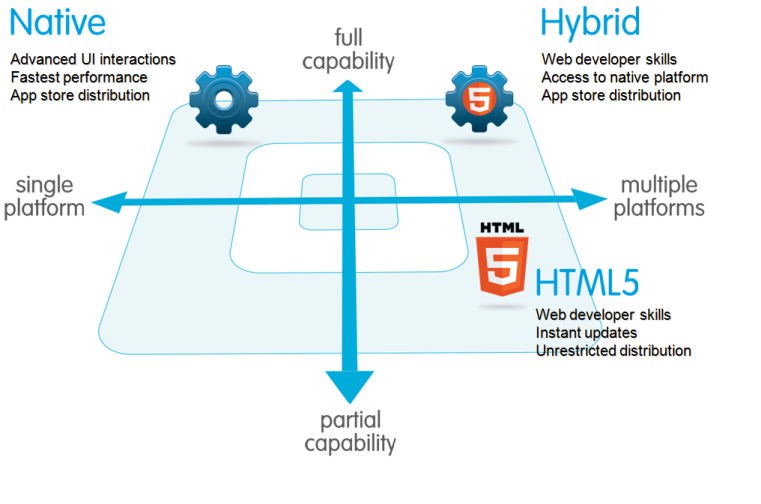
\includegraphics[width=0.9\textwidth]{../images/compare_hybrid_app.png}
  \caption[App híbrida]{App móvil híbrida (\href{https://developer.salesforce.com}{https://developer.salesforce.com}).}
  \label{fig:compare_hybrid_app}
  \end{center}
\end{figure}

Las principales ventajas de estas aplicaciones son:

\begin{itemize}
  \item \itembf{Bajo coste de desarrollo.}
  \item \itembf{Multiplataforma.}
  \item \itembf{Tiempo de desarrollo corto.}
  \item \itembf{Fácil distribución.}
\end{itemize}


\bigskip
Y lo que más nos interesa para este proyecto, sus desventajas:

\begin{itemize}
  \item \itembf{Rendimiento pobre.}
  \item \itembf{Escalabilidad baja.}
  \item \itembf{Diseño sujeto al diseño web.}
  \item \itembf{Acceso a las características especiales del hardware limitado.}
\end{itemize}


\bigskip
En un principio la aplicación que se desarrolló en el período de prácticas ICARO se planteó como una aplicación sencilla donde consultar conceptos y esquemas de las asignaturas. Los datos se consultarían desde una hoja de Google Drive común al departamento y se mostrarían en la aplicación directamente y por estas características, se .

A medida que avanzaba el desarrollo  y acercándose la fase final, el ``cliente'' planteó nuevas funcionalidades, topándonos con el primer problema: \textbf{la escalabilidad} de estas aplicaciones.



\subsection{Análisis del problema}
Una vez desarrollada esta aplicación, aunque en general quedamos contentos con el resultado, acusamos los siguientes problemas:

\begin{itemize}
  \item \itembf{No disponíamos de un servidor, toda la aplicación se ejecutaba en el cliente.}
  \item \itembf{Falta de base de datos.}
  \item \itembf{No se usa la API de Google Drive}
  \item \itembf{Acceso a Google Drive en cada sección de la aplicación}
  \item \itembf{Lentitud de acceso de datos en cada sección de la aplicación}
  \item \itembf{Mala elección de framework CSS, señales de obsoleto.}
\end{itemize}

\bigskip 
Solventar estos problemas, con el fin de iniciar un proyecto mejor planificado, con miras a una mayor escalabilidad analizando los requisitos presentes y los que pudieran surgir en un futuro, es la principal motivación para este proyecto. Aprovecharemos para mejorar la experiencia de usuario, ya que la lentitud de carga entre secciones era uno de los grandes problemas que hacían tediosa la consulta del contenido de la asignatura.

\bigskip
El primer paso importante es olvidar la tecnología móvil híbrida, que originó muchos problemas en el proyecto anterior y dividirlo en dos, una parte de desarrollo web y una parte de desarrollo móvil capaces de escalar sin problema. Nuestro proyecto se centrará en la aplicación web.


\section{Estado del arte}
Para abordar los problemas descritos y antes de realizar un análisis más profundo se hará un estudio de las tecnologías web que pueden sernos útiles en proyectos de este tipo.


\section{Elección de la tecnología}